%==============================================================================
\section{Algorithm}
\label{sec:algoritmo}
%==============================================================================

%==============================================================================
\subsection{Complexity Analysis}
\label{subsec:complexity}
%====================================================================

%==============================================================================
\subsection{Proposal}
\label{subsec:proposal}
%==============================================================================
A modelagem de um problema PSO é dividida em duas fases: definição do problema e definição da função aptidão. A primeira consiste em definir como o problema será codificado, ou seja, definir como a solução será representada. A segunda, em definir o quão \textit{boa} uma partícula será medida, ou seja, definir a função de aptidão.
Já para transformar o problema PSO em um algoritmo, é preciso definir a partícula e sua dimensão. Na abordagem adotada neste artigo, uma partícula representa um fluxo de trabalho e suas tarefas, e dimensão da partícula representa o número de tarefas no fluxo de trabalho. A dimensão de uma partícula serve para localizar sua posição no espaço, definindo o sistema de coordenadas. No exemplo do workflow do Café, a dimensão da partícula é quatro, sendo sua posição especificada por um sistema com quatro coordenadas.

Uma partícula movimenta-se num espaço limitado, denomina-se alcance. Na abordagem adotada neste artigo, o alcance é determinado pelo número de \emph{pools} de \emph{threads} disponíveis para executar a tarefa. Assim, o valor de uma coordenada no sistema de coordenadas, que define o espaço de movimentação da partícula, tem um alcance de 0 até o número máximo de \emph{pools} de \emph{threads} disponíveis. A parte inteira do valor de uma coordenada na posição de uma partícula corresponde ao número de \emph{pools} de \emph{threads} e representa o recurso computacional atribuído a uma tarefa definida por essa coordenada específica. Assim, a posição da partícula corresponde a um mapeamento da tarefa em recursos. 

Para o workflow do Café, valores para as quatro coordenadas(tarefas) do nosso sistema de coordenadas, no qual existem três recursos computacionais (\emph{pools} de \emph{threads} disponíveis), de forma que o valor de cada coordenada poderá variar entre 0 e 3. Há 4 tarefas para serem mapeadas, o que corresponde a dimensão 4 da partícula, portanto a posição da partícula terá 4 coordenadas. O índice da coordenada (de 1 a 4) corresponde a uma tarefa (de $t_1$ a $t_{4}$). O valor da coordenada é um número real de 0 a 3 , correspondendo ao número de recursos disponíveis para cada tarefa, com o máximo de 3 no nosso exemplo. Quando esse número inteiro é arredondado, é determinado o número de recursos disponíveis para cada tarefa. 
%Conforme o exemplo da Figura~\ref{fig:coordenadas}, a coordenada 1 da tarefa 1 tem valor igual a $1,3$ significando que para essa tarefa foi alocado 1 recurso, pois 1 é a parte inteira desse valor; a coordenada 2, corresponde a tarefa 2, tem valor de $ 2,0 $ indica que para a tarefa 2 foram alocados 2 recursos; e assim, sucessivamente até a coordenada 4.
%\begin{figure}[htb]
%\centering
%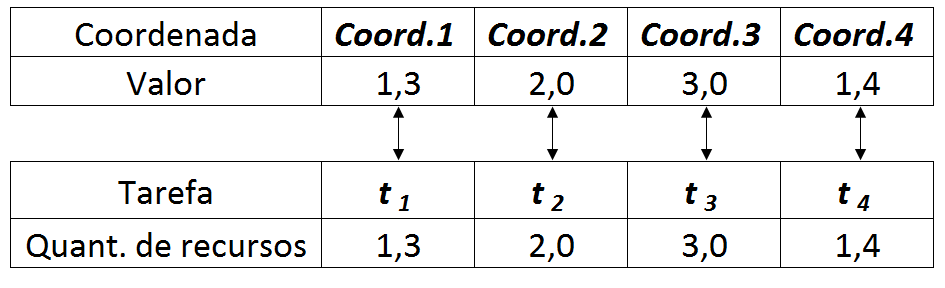
\includegraphics[scale=0.25]{./figs/coordenadas.png}
%\caption{Coordenadas da posição das partículas no espaço.}
%\label{fig:coordenadas}
%\end{figure}
A função de aptidão deve refletir os objetivos do problema de agendamento, pois ela é usada para determinar o quão boa uma determinada solução é. Nessa abordagem, ela é minimizada e seu valor será o tempo total de execução $TTE$ contido no agendamento $A$ derivado da posição da partícula. Considerando que o motor de execução é capaz de aumentar elástica e dinamicamente a quantidade de recursos, o modelo de aquisição oferecido pela computação em nuvem parece ilimitado, ou seja, não há um conjunto de recursos disponíveis que pode ser usado no algoritmo. A estratégia é definir um conjunto inicial de recursos que o algoritmo pode usar para explorar diferentes soluções e alcançar o agendamento. O tamanho desse conjunto será nossa restrição ${TR \le {\delta _r}} $, conforme a Equação~\ref{equa:problema}. Tal estratégia tem de refletir a heterogeneidade dos \emph{pools} de \emph{threads} (diferentes números de \emph{threads}) e oferecer opções suficientes de PSO, a fim de que seja produzida uma partícula adequada, ou seja, a solução. O conjunto de recursos inicial e limitado conterá os recursos que podem ser usados. Se esse conjunto é muito grande, o número de agendamento possíveis aumentará, assim como, o espaço de pesquisa explorado pelo PSO, tornando difícil para o algoritmo convergir e encontrar uma solução adequada~\cite{rodriguez2014}.

Para reduzir o tamanho do espaço de pesquisa, o qual será usado pelo PSO para encontrar um agendamento próximo do ótimo, considera-se um conjunto de recursos inicial $R_{inicial}$, composto por um $Pool$ de cada tipo, para cada tarefa em P; onde P é o conjunto que contém o número máximo de tarefas que podem ser executadas em paralelo para um dado fluxo de trabalho. O algoritmo selecionará o número e o tipo apropriados de $Pools$ para o motor de execução, dentro das opções contidas em $R_{inicial}$. Assim, reflete-se a heterogeneidade dos recursos computacionais e reduz-se o tamanho do espaço de busca, além de permitir mapear todas as tarefas que podem ser executadas em paralelo. O tamanho de $R_{inicial}$ seria igual a $\left| P \right|*n$, onde $n$ é o número de tipos de $Pools$ disponíveis, sendo ainda possível, que o PSO selecione mais de um recurso $\left| P \right|$, se necessário (a menos que $n = 1$).

O problema abordado possui a restrição  ${TR \le {\delta _r}} $, utiliza-se uma versão do PSO que incorpora uma estratégia para tratar restrições~\cite{deb2002}. Nela, sempre que duas soluções estão sendo comparadas e (\textit{i}) ambas as soluções forem viáveis, então a solução com melhor aptidão é selecionada; (\textit{ii}) se uma solução é viável e a outra não é, então a viável é selecionada; e finalmente, (\textit{iii}) se ambas as soluções são inviáveis, aquela que violar menos a restrição é selecionada. No último caso, implica que uma medida de quanto uma solução viola a restrição precisa ser encontrada. O problema define o valor de violação de restrição de uma solução $\delta_k $, a restrição pode ser atribuída a limitação de recursos que se deseja contratar na computação em nuvem ou simplesmente e a quantidade de \emph{threads} físicas das máquinas que irão ser utilizadas na execução da solução de integração. Uma solução do PSO que utilize recursos próximos de $\delta_k$ será preterida em relação a uma solução menos recursos.

O Algoritmo~\ref{algoritmo-agendamento} apresenta o pseudo-código para mapear a posição de uma partícula em um agendamento. O conjunto de recursos $R$ para serem alocados e o conjunto de mapeamentos $M$ de tarefas para recursos são inicializados sem elementos, ou seja, vazios, e tempo total de execução $TTE$ é inicializado com o valor zero. Na sequência, o algoritmo estima o tempo de execução de cada tarefa do fluxo de trabalho para todo o recurso ${r_i} \in {R_{inicial}}$. A representação é uma matriz em que as linhas representam as tarefas, as colunas representam os recursos e a entrada $ TempoExec[i,j] $ corresponde ao tempo gasto para executar a tarefa $t_i$ no recurso $r_j$, calculado conforme a Equação~\ref{equa:tempo-execucao}. O próximo passo é o cálculo ou atribuição da matriz de tempo de transferência de dados, ou tempo de espera na fila de tarefas, o qual assume-se que está sendo obtido por um procedimento, não tratado nesse trabalho, tal como por uma ferramenta de monitoramento. Essa matriz é representada como uma matriz de adjacência ponderada do workflow DAG, onde a entrada $ TempoTransfer[i, j]$ contém o tempo que leva para transferir os dados de saída da tarefa $t_i$ para a tarefa $t_j$ e esse valor é zero sempre que $i =j$ ou não há aresta direcionada conectando $t_i$ (tarefa pai) e $t_j$ (tarefa filha). 
%A Figura~\ref{fig:matrizes} exemplifica essas matrizes para o workflow do Café.
%\begin{figure}[htb]
%	\centering
%	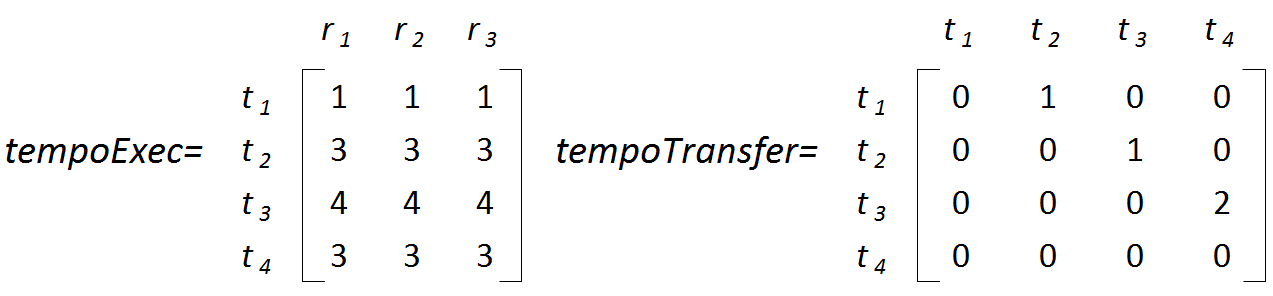
\includegraphics[scale=0.2]{./figs/matrizes-h.png}
%	%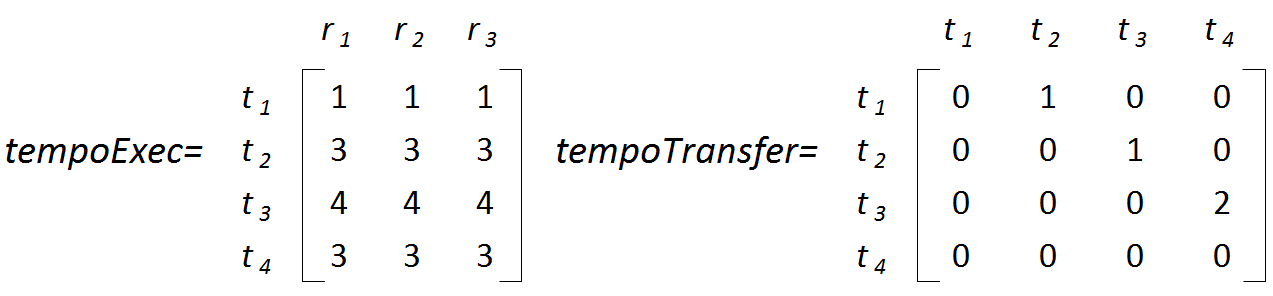
\includegraphics[width=\linewidth]{./figs/matrizes-h.png}
%	\caption{Matrizes Tempo de Execução e de Transferência.}
%	\label{fig:matrizes}
%\end{figure}
De posse dessas informações, o algoritmo inicia determinando a posição da partícula e construindo o agendamento. Para isso, itera para toda $ i $ do \textit{array} de posição $pos$ e atualiza $ R $ e $ M $. Primeiro, determina a tarefa e o recurso que está associado à coordenada atual e seu valor. A estratégia usada para isso é a descrita anteriormente, a qual indica que a coordenada $ i $ corresponde à tarefa $t_i$ e seu valor $pos[i]$ corresponde ao recurso $  {r_{pos[i]}} \in {R_{inicial}} $. Encontrados os componentes, $ {t_i} $ e $ {r_j} $, de uma tupla de mapeamento $ m_{{t_i}}^{{r_j}} $, o algoritmo calcula os demais, o tempo de inicio $ TIn{i_{{t_i}}} $ e tempo de finalização $TFi{n_{{t_i}}}$ da tarefa.

O valor de tempo de início $ TIn{i_{{t_i}}} $ diferencia-se em duas situações. Na primeira, a tarefa não tem tarefa pai e, portanto, pode começar a ser executada, assim que o recurso alocado para ela $r_{pos[i]}$ estiver disponível, o que ocorrerá quando o referido recurso terminar a execução que estiver em andamento. Na segunda situação, a tarefa tem um ou mais pais e, nesse caso, além de esperar que o recurso para ela alocado esteja disponível, também terá que aguardar pelo término da execução das suas tarefas pai, além do tempo de transferência dos dados.

O valor de $TFin_{t_i}$ é calculado baseado no tempo total de processamento e no tempo de início da tarefa. Para determinar o tempo de processamento $TP_{{t_i}}^{r_{pos[j]}}$, é necessário calcular o tempo de execução e o tempo de transferência. O primeiro é $TempoExec[i,pos[i]]$, enquanto o último é calculado pela soma dos valores do tempo de transferência $TempoTransf[i,filha(i)]$ para toda tarefa filha $t_{filha(i)}$ de ${t_i}$, que está mapeada para rodar em um recurso diferente de $r_{pos[i]}$. Esses dois valores são então somados para obter $TP_{{t_i}}^{r_{pos[j]}}$, como definido na Equação~\ref{equa:tempo-processamento}. Por fim, o valor de $TFin_{t_i}$ é obtido pela subtração de $TIni_{t_i}$ de $TP_{{t_i}}^{r_{pos[j]}}$.
Calculados os elementos de $ m $, adiciona-se recurso para $R$, se necessário. 
Quando o algoritmo termina de processar, cada coordenada do vetor posição, $R$ conterá todos os recursos necessários e os tempos de início e finalização. Além disso, o mapeamento completo das tarefas para os recursos estará em $M$ e cada tarefa terá um recurso atribuído a ela e o tempo estimado de início e o de término. Com essas informações o algoritmo pode calcular o $TTE$  associado a solução atual, conforme Equação~\ref{equa:tempo-processamento}. Nesse ponto, o algoritmo calculou $R$, $M$ e $TTE$ e poderá construir e apresentar o agendamento associado para essa posição da partícula.
\begin{algorithm}
	\caption{Geração de agendamento}
	\ {\textbf{Entrada:} Conjunto de fluxo de trabalho de tarefas $ T $}
	
	\ {Conjunto Inicial de recursos $ R_{inicial} $}
	
	\ {Um array  $pos[{\left| T \right|}]$ representando a posição da partícula}
	
	\ {\textbf{Saída:} Um agendamento $ A $}
	
	\begin{algorithmic}[1]
		
		\State { $ \texttt{R} = \emptyset, \texttt{M} =  \emptyset, TTE = 0 $ } \Comment {Inicializa componentes}
		\State { Calcula $ {{TempoExec[}}\left| T \right| \times \left| {{R_{inicial}}} \right|] $}
		\State { Calcula $ {{TempoTransf[}}\left| T \right| \times \left| T \right|] $}
		\For{$ i $}{0}{$\left| T \right|-1$} 
		\State {$ t_i = T[i], r_{pos[i]} = \texttt{R}_{inicial}[pos[i]]  $}
		\If {$ {t_i}$ não tem pai}
		\State {$ TIni_{t_i} = TFin_{r_{pos[i]}} $}
		\Else
		\State {$ TIni_{t_i} = (\max {\{TFin_{t_{pai}}:t_{pai}[ \in pais(t_i) \}},TFin_{r_{pos[i]}}) $}	
		\EndIf
		\State {$ exe = tempoExec \left[ i \right]\left[ {pos\left[ i \right]} \right] $}
		\For {cada filha $ t_{filha} $ de $ t_i $}
		\If {$ t_{filha}$ é mapeada para um recurso diferente de  $r_{pos[i]} $}
		\State { $ trasfer+ = TempoTransf[i][c] $}	
		\EndIf	
		\EndFor
		\State {$TP_{{t_i}}^{r_{pos[j]}} = exe + transf$}
		\State {$ TFin_{t_i} = TP_{{t_i}}^{r_{pos[j]}} - TIni_{t_i}  $}
		\State {$ m_{{t_i}}^{{r_{pos[j]}}} = (t_i,r_{pos[i]},TIni_{t_i},TFin_{t_i})  $}
		\State {$ \texttt{M} = \texttt{M} \cup \{ m_{{t_i}}^{{r_{pos[i]}}}\}   $}
		\If {$ {r_{pos[i]}} \notin \texttt{R}  $}
		\State {$ \texttt{R} = \texttt{R} \cup {r_{pos[i]}}  $}
		\EndIf
		\EndFor 
		\State { Calcula $ TTE $ conforme Equação~\ref{equa:tempo-total-execução} }
		\State {$ A = (R, M, TR, TTE) $}
	\end{algorithmic}
	\label{algoritmo-agendamento}
\end{algorithm}
Finalmente, os Algoritmos~\ref{algoritmo-pso} e \ref{algoritmo-agendamento} são combinados para o agendamento próximo de ótimo. Na linha 4 do Algoritmo~\ref{algoritmo-pso}, em vez de calcular o valor de aptidão da partícula, gera-se o agendamento, conforme Algoritmo~\ref{algoritmo-agendamento}. Em seguida, usa-se o $ TTE $ como valor de aptidão nas etapas seguintes e é introduzido o mecanismo de manipulação de restrição, tal que  ${TR \le {\delta _r}} $.  